
\documentclass[11pt, a4paper, preprint]{article}
\usepackage{outline}
\usepackage{float}
\usepackage{graphicx}
\usepackage{color}
\usepackage{amsmath}
\usepackage{cite}
\graphicspath{ {Figs/} }

\usepackage[T1]{fontenc}
\usepackage[utf8]{inputenc}
\usepackage{authblk}
\newcommand{\tcr} { \textcolor{red} }


\title{Multiscale Modeling of the Paradoxical Roles of the Immune System in EMT-Mediated Cancer}
\author{}

\renewcommand\Authands{ and }


\begin{document}
\maketitle


\section*{Abstract}
%% Basic Introduction (1-2 sentences)
Preceding tumorigenesis and throughout the lifetime of a tumor, the immune system is engaged in complex sets of interactions in and around the tumor.
%% More Detailed Background (2-3 sentences)
These are regulated by the tumor microenvironment (TME) in myriad ways. Moreover,  epithelial cell plasticity impacts disease incidence and progression via processes of epithelial-to-mesenchymal transition (EMT).
In turn, both the tumor and the immune system exert substantial influence over the TME in competition to influence the fate of the host.
%% General Problem (1 sentence)
Determining the factors and mechanisms underpinning these complex interactions remains an important task for cancer immunotherapy.
%% Summarizing Main Result (1 sentence)
%Here, we seek to understand how interplay between the tumor, the immune system, and EMT can determine the outcome of cancer.
%% The Main Result (2-3 sentences)
We developed a multiscale agent-based model to describe the interplay between three components: the tumor (or pre-tumor cells), the immune system, and EMT.
The model revealed a \tcr{non-monotonic relationship} between the cell cycle times associated with the mesenchymal phenotype and the probability of tumorigenesis, identifying a critical growth rate that maximizes cancer-free survival. In comparison, increasing the immune-evasiveness of the mesenchymal phenotypes always led to poorer prognosis. Moreover, encouraging
%\tcr
the TME
towards a pro-EMT state also benefits the tumor.
%% Putting into a More General Context (1-2 sentences)
Together, these results indicate that the joint regulation of the TME by the immune system and the tumor itself provides possible targets for future cancer therapies, in particular cancers such as pancreatic cancer in which EMT is speculated to play a role.

%%%%%%%%%%%%%%%%%%%%%%%
%                    INTRODUCTION                    %
%%%%%%%%%%%%%%%%%%%%%%%


\section{Introduction}
Immunotherapy is slowly revolutionizing cancer therapy. New breakthroughs in the field begin to produce new therapies that have had a significant impact on patient health and survival\cite{pardoll2012blockade}\cite{restifo2012adoptive}.
% A More examples? Reviews or non-reviews? Explain some of the examples?
%AM I will add a few 
%There are myriad untapped avenues by which scientists can further explore the role of the immune system in regulating and combatting cancer;
In addition to direct cell-cell interactions between immune and cancer cells, the means by which immune cells interact with and modulate the tumor microenvironment (TME) is an important \tcr{research} area.
Immune cells can be understood as one constituent of the TME: responding to the environment's inflammatory signals, fighting the mutated cells present, and then restoring homeostasis in that local context\cite{de2006paradoxical}.
Understanding each step in this immune cascade in the context of the TME will be necessary in order to fully explore and exploit all options of immunotherapy.

\tcr{Still need to address Qing's comments on this paragraph:}

The tumor interacts with the immune system by initiating the sequence of events that results in the activation of the adaptive immune response.
It accomplishes this by presenting antigens that innate immune cells recognize and carry to lymph nodes to activate, among other things, T cells.
Also, tumor cells engage in certain cellular processes that shape the TME and thus impact the immune system.
In particular, tumor cells release transforming growth factor beta (TGF-$\beta$) that creates a tumor-supportive environment by shifting the immune balance to being immunosuppressive via enhancing activation of Treg cells.

This particular cytokine is also a driver of the epithelial-to-mesenchymal transition (EMT) and through generating TGF-$\beta$ the tumor creates a more mesenchymal phenotype within the TME.
\tcr{I think this is where I would add which types of cancer most likely to be affected by EMT. But which? And what sources?}
In this way, the tumor shifts the balance of local environment along the EMT spectrum.

The immune system has several competing interactions with the tumor.
While the cytotoxic immune cells, NKs and cytotoxic T cells (CTLs), seek out and lyse tumor cells, the regulatory branch of the immune system, which will be accounted for by Tregs in our model, slows down the effector functions of these other cells. % Make sure there's some ref for immune clearing tumor
% Also, add that as immune cells clear tumor cells, they become deactivated and give source

In relation to EMT, the Tregs of the immune system drive the EMT process by releasing TGF-$\beta$ upon arriving at the tumor site\cite{terry2017new}.
In this way, just as the tumor cells push the TME towards a mesenchymal phenotype, so too do the Tregs.

Epithelial-to-mesenchymal transition (EMT) describes the (reversible) cell plasticity process by which epithelial cells transition into mesenchymal cells.
While the epithelial cells often stay bound together in layers, mesenchymal cells have gained motility and even stem-like properties\cite{nieto2016emt}.
Recent work has revealed the intriguing possibility that there are intermediate cell states along the EMT spectrum with each state having its own unique properties\cite{hong2015ovol2}.
Such intermediate states have the potential of being connected to tumor initiation, progression, and metastasis\cite{nieto2016emt}.
While there might be many other characteristics distinctive of mesenchymal cells that need further exploration, two qualities of mesenchymal cells are particularly relevant in the context of cancer and the immune system:
1) mesenchymal cells are less susceptible to immune clearance\cite{terry2017new} and
%
2) mesenchymal cells proliferate at a slower rate. \tcr{Ref}
 %A Adam said he had a reference in mind for this.

The immune evasiveness of mesenchymal cells is well-established with even a functional cause for this phenomenon.
As a cell is being targeted by cytotoxic immune cells for clearance, a physical connection between the two cells must be created in order to precipitate the lysing event.
This immunological synapse, however, is dependent upon the surface proteins of the target cell, and in the case of mesenchymal cells there is preliminary evidence that these surface markers are down-regulated in such a way that the immune synapse is more difficult to form\cite{terry2017new}.
There are also other structural changes that take place in mesenchymal cells that could contribute to this refractory nature towards immune clearance.
Regardless, the evidence currently demonstrates a ``slipperiness'' of mesenchymal cells in regards to immune lysing.
We will refer to this as mesenchymal immune evasion, or MIE.

The other facet of mesenchymal cells is their slower proliferation rate, and this is tied to the observation that mesenchymal cells often express a more stem-like phenotype.
Indeed, even in healthy tissue, this is readily observed and seen as a useful mechanism for homeostasis as epithelial cells can transition to mesenchymal, stem-like cells under appropriate conditions. \tcr{Ref}
While many qualities are associated with being stem-like, we choose to focus on a reduced proliferation rate. \tcr{Ref}
Cancer cells are well-known for achieving unregulated proliferation, so exploring a subset of cancer cells with decreased proliferation could provide intriguing new results.
In our model, we refer to this property as mesenchymal growth arrest, or MGA.

Recent work on cancer-immune interactions has shown that the inflammatory conditions of the TME can play large and sometimes surprising roles in tumor growth.
For example, a mathematical model was developed to couple the inflammatory state of the TME with the cell cycles of the stem cells by increasing proliferation, decreasing apoptosis, and enhancing DNA damage that leads to mutations\cite{guo2017multiscale}.
The work shows that while inflammation does have an oncogenic effect, it can also have an onco-protective role as periods of mild inflammation are better at preventing cancer than periods of no inflammation in patients that have intermittent bouts of severe inflammation.
However, the aspect of the model that included the immune system is minimal and the connection with EMT is not included.
%However, the aspect of the model that included the immune system was minimal: regardless of the inflammatory environment, any cells with sufficient pathway mutations (2 in their model) had a fixed probability of being cleared by the metabolism-immune balance response. 
Here, we include a more robust immune module and explore how this immune module will improve our understanding of inflammatory effects on the tumor, and also include the epithelial-mesenchymal axis.
%In addition, we explore an extra component of Guo's stem cells: where they lie on the epithelial-mesenchymal axis.
Such additions will allow us to explore the interactions of the tumor, the immune system, and the epithelial-mesenchymal spectrum as well as the effects of the TME on these interactions.
%We will also study the effects of the TME on these interactions.

Next, we introduce the model modularly, which is appropriate given its multiscale and hybrid nature.
We then perform sensitivity analysis and identify parameters that are crucial for the progression to tumorigenesis.
We analyze the competing effects of EMT and of the immune system on tumorigenesis and find that EMT intricately regulates tumorigenesis: under certain regimes a careful balance of EMT- and immune-driven process can significantly prolong cancer-free survival.


%%%%%%%%%%%%%  INTRO PARAGRAPH GRAVEYARD %%%%%%%%%%%%%%%%

%They release cytokines that alter the extracellular matrix, promote angiogenesis, and create an inflammatory environment.
%This last one, in particular, results in the impairment of cytotoxic capabilities of immune cells.
%Through 
%
% its presence and by the cellular processes it engages in that result in shaping the TME.
%On the one hand, the mutated DNA of tumor cells results in these cells being recognized as foreign by members of the innate immune system such as natural killer (NK) cells and dendritic cells.
%It is then these cells that initiate the cascade of cytokines that result in the full activation of the body's immune system to fight the non-self cells.
%On the other hand, the tumor cells actively work to shape the immune response that the body launches.
%This is accomplished through its own set of cytokines, such as transforming growth factor beta (TGF-$\beta$), that work to create a tumor-supportive environment, including shifting the immune balance to be immunosuppressive by enhancing the recruitment of Treg cells. Since TGF-$\beta$ is also a driver of EMT, then through direct release of TGF-$\beta$ and recruitment of TGF-$\beta$-secreting Treg cells, cells of the tumor and the surrounding tissue are driven towards a more mesenchymal profile. 

%In quantifying this property, we use the model parameter `mesenchymal growth arrest', MGA.
%This choice is less about associating this property with quiescence and more about creating a simple name that easily, if not roughly, captures the essence of what is being modeled.
%For example, while mesenchymal proliferation reduction might be a more accurate term, thinking in terms of a negative formulation adds one additional twist to accurately interpreting results which we felt was more detrimental than the possible confusion of invoking ``quiescence.''

%This plays an important yet complicated role in tumor initiation, progression, and metastasis\cite{nieto2016emt}. % References more specific to this claim might be in this paper's references. 
%As mesenchymal cells often exhibit stem-like properties, their existence in a tumor has been tied to the initiation and progression of cancer\cite{nieto2016emt}. % References more specific to this claim might be in this paper's references.
%Also, due to their motility, some have viewed them as a natural precursor to metastasis\cite{alderton2012metastasis}. 
%
%Conversely, the mesenchymal cells in the tumor downregulate certain surface markers making it more difficult for cytotoxic immune cells to form the immune synapse necessary to lyse the cancer cell\cite{terry2017new}.
%Taking these three aspects together, all influencing the others, we can consider the simple diagram in Figure \ref{fig:3PartFig} and see just how much potential there is for exploring all these relationships.
%Each of these three pieces will be briefly explored in turn for how they will influence one another.









%%%%%%%%%%%%%%%%%%%%%%%
%                         METHODS                        %
%%%%%%%%%%%%%%%%%%%%%%%

% This paragraph needs to find a home in this section somewhere

\section{Methods}
To address the questions around the relationships among cancer, the immune system, and EMT, we extended the multiscale, agent-based model \tcr{REF} to include an immune module and an EMT axis for the tissue cells.
The agents in the model are the tissue cells with tumorigenic potential.
They can either be mutation-free, or have any combination of three possible pathway mutations.
These three pathways are the three components within each cell in Figure \ref{fig:ModelIntro}A.
If the pathway is mutated, the component is colored red and has an `X'.
A single mutation is sufficient for the cell being counted as a mutant cell.

We model the immune cells as discrete variables but as one collective, in other words they are not agents themselves.
The cytokine TGF-$\beta$ is a continuous variables within the tumor microenvironment (TME).
It is worth noting that there is no spatial aspect to this model.
In doing this, we are assuming that cells are well-mixed as are all the relevant cytokines and other molecules acting on the system.
Finally, tissue cells can be labeled either epithelial or mesenchymal, and this labeling can change over time and depends both on the TME and the internal workings of each individual cell.
While the score is continuous, a threshold determines if a given cell is labeled as epithelial or mesenchymal.
In Figure \ref{fig:ModelIntro}A, the EMT labeling is given by the color of the cell.
Even though each cell does have an EMT score on a spectrum of values, only the labeling influences its interactions in the model.

\subsection{Tissue Cells}\label{TissueCells}
The tissue cells at all times have associated with them two important quantities: which combination of mutations they carry and an EMT score.
The model has three pathways that have the potential to mutate over the course of a simulation.
There is a proliferation pathway that when mutated increases the probability of the cell proliferating.
There is an apoptosis pathway that when mutated decreases the probability of the cell undergoing apoptosis.
There is an immune evasion pathway that when mutated decreases the probability that an immune cell can effectively clear the mutated cell.
% It might be nice to have a table to summarize this information?
The EMT score will be exposited in Section \ref{EMT}. % make sure this is really the best decision


%Add differential equations? % Should this be done here or where I have it later?

\subsection{The Immune System}\label{ImmuneSystem}
The immune system is modeled as having three active immune cell types: NKs, CTLs, and Tregs.
The NKs and CTLs act on the system by recognizing mutated cells and clearing them.
Upon successful clearance, they themselves are then deactivated and removed from the immune population.
Tregs act on the system by suppressing the effector functions of NKs and CTLs, making it less likely they can clear mutated cells.
In addition to this, Tregs release TGF-$\beta$ which further shapes the TME by pushing tissues cells more towards a mesenchymal phenotype.

\subsection{EMT}\label{EMT}
Each tissue cell has an EMT score between 0 and 1.
When the score is above a fixed threshold value, the cell is labeled as mesenchymal.
Otherwise, it is below the threshold and labeled as epithelial.
For the purposes of the model, a cell in an epithelial state is considered in the base state, and one in a mesenchymal state will have some of its parameters updated.
In particular, mesenchymal cells benefit from increased immune evasion but suffer from decreased proliferation.
Note, that because the immune system can only clear mutated cells, the increased immune evasion only benefits mutated mesenchymal cells.

\subsection{Model Simulation}

\subsubsection{Initial conditions} Every model run starts with a fixed amount of cells, $N_0$.
However, different parameter values will lead to different steady states for the population of tissue cells.
In light of this, a warmup period of ~1000 cell cycles is used in which time no mutations are allowed to happen.
Thus, the only immune cell present is NKs.
After the warmup cycles are complete, a mutagenic event is simulated in which all the tissue cells experience a random increase in their probability to mutate.
From then on, a cell which proliferates either mutates or increases its probability of mutating later on.

\subsubsection{Tissue cell fate}
During each cell cycle, every cell randomly is assigned a cell fate from the following options:
\begin{itemize}
\item proliferation
\item apoptosis
\item immune clearance (by NKs or CTLs)
\item rest in $G_0$
\end{itemize}

For each cell, a weight is chosen for each option and these are normalized to probabilities which then are used to randomly determine what each cell does during the cell cycle.

\paragraph{Proliferation}
There are four factors that contribute to the probability that a cell will proliferate.
The first is a base proliferation probability that all cells have, $p$.
Second, if the cell has a mutation in the proliferation pathway, then the weight for proliferation is proportionally increased by $\text{prolif}_{\text{up}}$.
Third, if the cell is mesenchymal, then the weight for proliferation is proportionally decreased by $m_{GA}$, which stands for mesenchymal growth arrest.
Fourth, there is a negative feedback of the cells on their own proliferation which is quantified by a Hill factor as a function of the tissue cell population, $N$.
In total, the weight for proliferation is given by

$$ p_{prolif} = p(1+\delta_{\text{PM}}\text{prolif}_{\text{up}})(1-\delta_{MES}m_{GA})\frac{N_0}{N_0+N} $$

\paragraph{Apoptosis}
There are two factors that contribute to a cell's weight for undergoing apoptosis.
There is a basal apoptosis rate that all cells experience, $d$ for death.
Second, if the cell has a mutation in the apoptosis pathway, then the weight for undergoing apoptosis is proportionally decreased by $\text{apop}_{\text{down}}$.
In total, the weight for apoptosis is given by 

$$ p_{apop} = d(1-\delta_{\text{AM}}\text{apop}_{\text{down}}) $$

\paragraph{Immune Clearance}
For both NK clearance and CTL clearance, the weights are built with the same factors but have different parameter values for NK and CTLs.
First of all, the cell needs to be mutated, $\delta_M$.
Second, there is a Hill factor that captures the probability of an immune cell finding and interacting with the given tissue cell.
Third, NKs and CTLs have their own efficacy parameters, $E_{\text{NK}}$ and $E_{\text{CTL}}$, which can be understood as the weight for immune clearance given an immune cell has found the mutated cell.
Fourth, there is a decreasing Hill factor based on the number of Treg cells present.
Finally, there are two factors that proportionally decrease the weight of immune clearance depending on if the cell has an immune evasion mutation or if it is mesenchymal.
In total, the weight of NK clearance is given by

$$ p_{\text{NK}} =\delta_M \frac{\text{NK}}{N/N_{1}+\text{NK}}  \frac{E_{\text{NK}}}{1+\text{Treg}/\text{Treg}_{\text{EC50}}} (1-\delta_{IEM}\text{IE}_{\text{up}})(1-\delta_{MES}m_{\text{IE}}) $$
% Should I worry about the order in which these appear? Rearranging would make the formula look better, but the order I have introduced them makes the most sense.
% Also, any thoughts on NK, CTL, Treg not being italicized? While other capital letters are?

A similar formula holds for CTLs with only the number of CTLs and their efficacy being different from the above equation.


\paragraph{Rest in $G_0$} 
The weight associated with quiescence is taken as 1 except in the case of Mesenchymal cells.
For Mesenchymal cells, the weight lost to proliferation is added to the weight of quiescence.
Hence, the weight of quiescence is given by

$$ p_{rest} = 1 + \delta_{\text{MES}}p(1+\delta_{\text{PM}}\text{prolif}_{\text{up}})m_{GA}\frac{N_0}{N_0+N} $$ 

The reason for adding that term is due to the understanding that overall mesenchymal cells proliferate less as individual cells rest longer in the $G_0$ phase.

\subsubsection{Completing the Cell Cycle}
After the cell fates are determined and the results reflected in the system, there are a few things that happen before the system moves on to a new cell cycle.
First, the NK and CTL populations are reduced by the number of mutated cells they cleared.
This represents the fact that individual immune cells lose efficacy as they carry out their effector functions. 
All proliferating cells have a nonzero probability of undergoing a pathway mutation.
If they do, one is randomly chosen among the three pathways and the pathway in that cell mutates.
If the cell does not undergo a mutation, then its probability of mutation during subsequent cell cycles increases. 
Then, the EMT values for each cell is updated.
This depends on the cells current EMT score and how much TGF-$\beta$ is currently in the system.
Each cell receives an amount of TGF-$\beta$ given by

%$$ \text{TGFB}_i = H(\text{TGFB}/N) + X_i, \quad X_i \sim N(0,\sigma^2)$$

$$ \text{TGFB}_i = \frac{\text{TGFB}_{max}}{N}\frac{\text{TGFB}/\gamma_{EC50}}{1+\text{TGFB}/\gamma_{EC50}}+ X_i
, \quad X_i \sim N(0,\sigma^2)$$
The summand on the left divides up the total TGF-$\beta$ among all $N$ cells evenly and a Hill function on this quantity determines how much TGF-$\beta$ each cell thus receives.
Then, some randomness is introduced by the independent and identically distributed variables $X_i$where $\sigma$ is a parameter in the model.
If this quantity is large enough, relative to the EMT score of the cell, then the cell will undergo EMT and its EMT score will increase.
If not, then the cell undergoes the reverse process, MET, and its EMT score will decrease.
Each cell then is relabeled as either epithelial or mesenchymal depending on its new EMT score and whether it is below or above the mesenchymal threshold.
Thus, there are two main factors that determine if a cell will end a cell cycle as mesenchymal: quantity of TGF-$\beta$ in the system and the current EMT score of the cell.

Next, the amount of TGF-$\beta$ for the next cell cycle is determined by the number of mutated cells, $M$, and the number of Treg cells, each one producing a fixed amount of TGF-$\beta$. It is given by

$$ \text{TGFB} = \text{tgfb}_{\text{mut}}M + \text{tgfb}_{\text{Treg}}\text{Treg}$$ % clear that M is number of mutants, right?

Finally, the immune populations are updated.
For the NKs, they obey the following differential equation:
 
$$ \text{NK}' = \sigma_{\text{NK}} - d_{\text{NK}}\text{NK} $$

which is discretized to
 
$$ \text{NK}_{k+1} = \left (\text{NK}_k-\frac{\sigma_{\text{NK}}}{d_{\text{NK}}} \right )\exp(-d_{\text{NK}}\Delta t)+\frac{\sigma_{\text{NK}}}{d_{\text{NK}}} $$


%%%% Which of these two paragraphs is better? Currently the intro does not mention APCs and I don't think I need to go into that, especially when APC_k = \tilde{M}_k
For CTLs and Tregs, they rely on mutant cells being cleared before they can be activated.
Let $\tilde{M}_k$ represent the number of mutant cells cleared by the immune system during cell cycle $k$.
In addition, Treg recruitment is upregulated by TGF-$\beta$, which will be incorporated via a Hill function.
We choose the following differential equations to govern the CTL and Treg populations:

\begin{align*}
\text{CTL}' & = \sigma_{\text{CTL}}\tilde{M} - d_{\text{CTL}}\text{CTL} \\
\text{Treg}' & = \sigma_{\text{Treg}}\tilde{M} \frac{\text{TGFB}}{1+\text{TGFB}/\text{EC50}}- d_{\text{Treg}}\text{Treg}
\end{align*}

Discretized, these are:

\begin{align*}
\text{CTL}_{k+1} & = & \left (\text{CTL}_k-\sigma_{\text{CTL}}\tilde{M}_k/d_{\text{CTL}}\right )\exp(- d_{\text{CTL}}\Delta t) + \sigma_{\text{CTL}}\tilde{M}_k/d_{\text{CTL}}\\
\text{Treg}_{k+1} & = & \left (\text{Treg}_k-\frac{\sigma_{\text{Treg}}\tilde{M}_k}{d_{\text{Treg}}} \frac{\text{TGFB}}{1+\text{TGFB}/\text{EC50}}\right )\exp(-d_{\text{Treg}}\Delta t)+\\
& & \frac{\sigma_{\text{Treg}}\tilde{M}_k}{d_{\text{Treg}}} \frac{\text{TGFB}}{1+\text{TGFB}/\text{EC50}}
\end{align*}

\subsubsection{Progression and tumorigenesis}
At the end of each cell cycle, the proportion of tissue cells that are mutated is calculated, and if it is above a certain threshold, a tumorigenic event is recorded and the patient is determined to have cancer.
The Time to Cancer is given as the time from the start of the simulation, not including warmup, until tumorigenesis.
Simulations run until either a tumorigenic event is recorded or until the maximum number of cycles has been reached.

\subsection{Parameter Sensitivity Analysis}
To identify a subset of the parameters to focus on, we used the Morris method, a one-step-at-a-time global sensitivity analysis.
The algorithm runs the model numerous successive times, changing exactly one parameter each run\cite{morris1991factorial, sohier2014improvement}.
Each model run involved 1000 patients and the value returned was the area under the survival curve.
We ran the algorithm by sampling at 30 points in parameter space and then changing each parameter one time at each point.
In the implementation by Sohier, they recommend using at least 10 points\cite{sohier2014improvement}.

To determine which points in parameter space to sample at, we had to create distributions on all parameter values.
To do this, we derived many parameters from existing literature and the rest we made reasoned predictions.
For example, many previous studies have established the parameters of immune population dynamics such as recruitment and death rates\cite{de2014modeling}.
Because our model only works with on the order of $10^2$ tissue cells whereas an actual tumor would have on the order of $10^9$ cells\cite{de2014modeling}, we scaled the parameters so the immune populations would also be proportionately reduced.
That is, for instance, how we ended up with NK cells having a steady state population of 10 cells in the model.

Once we had these parameter values, we created Gaussian distributions centered at these values with large variances and truncated at 0.
Some of the parameters were also truncated to the right because they represented a proportion, such as MIE and MGA, or because we simply wanted to keep the values within a reasonable range, such as the inflammation low and high duration parameters.
The variances were chosen as twice the mean to get a large spread of values.
%%%%%%%%%%%%%%%%%%%%%%%
%                          RESULTS                         %
%%%%%%%%%%%%%%%%%%%%%%%

\section{Results}

\begin{figure}[H]
\center
\frame{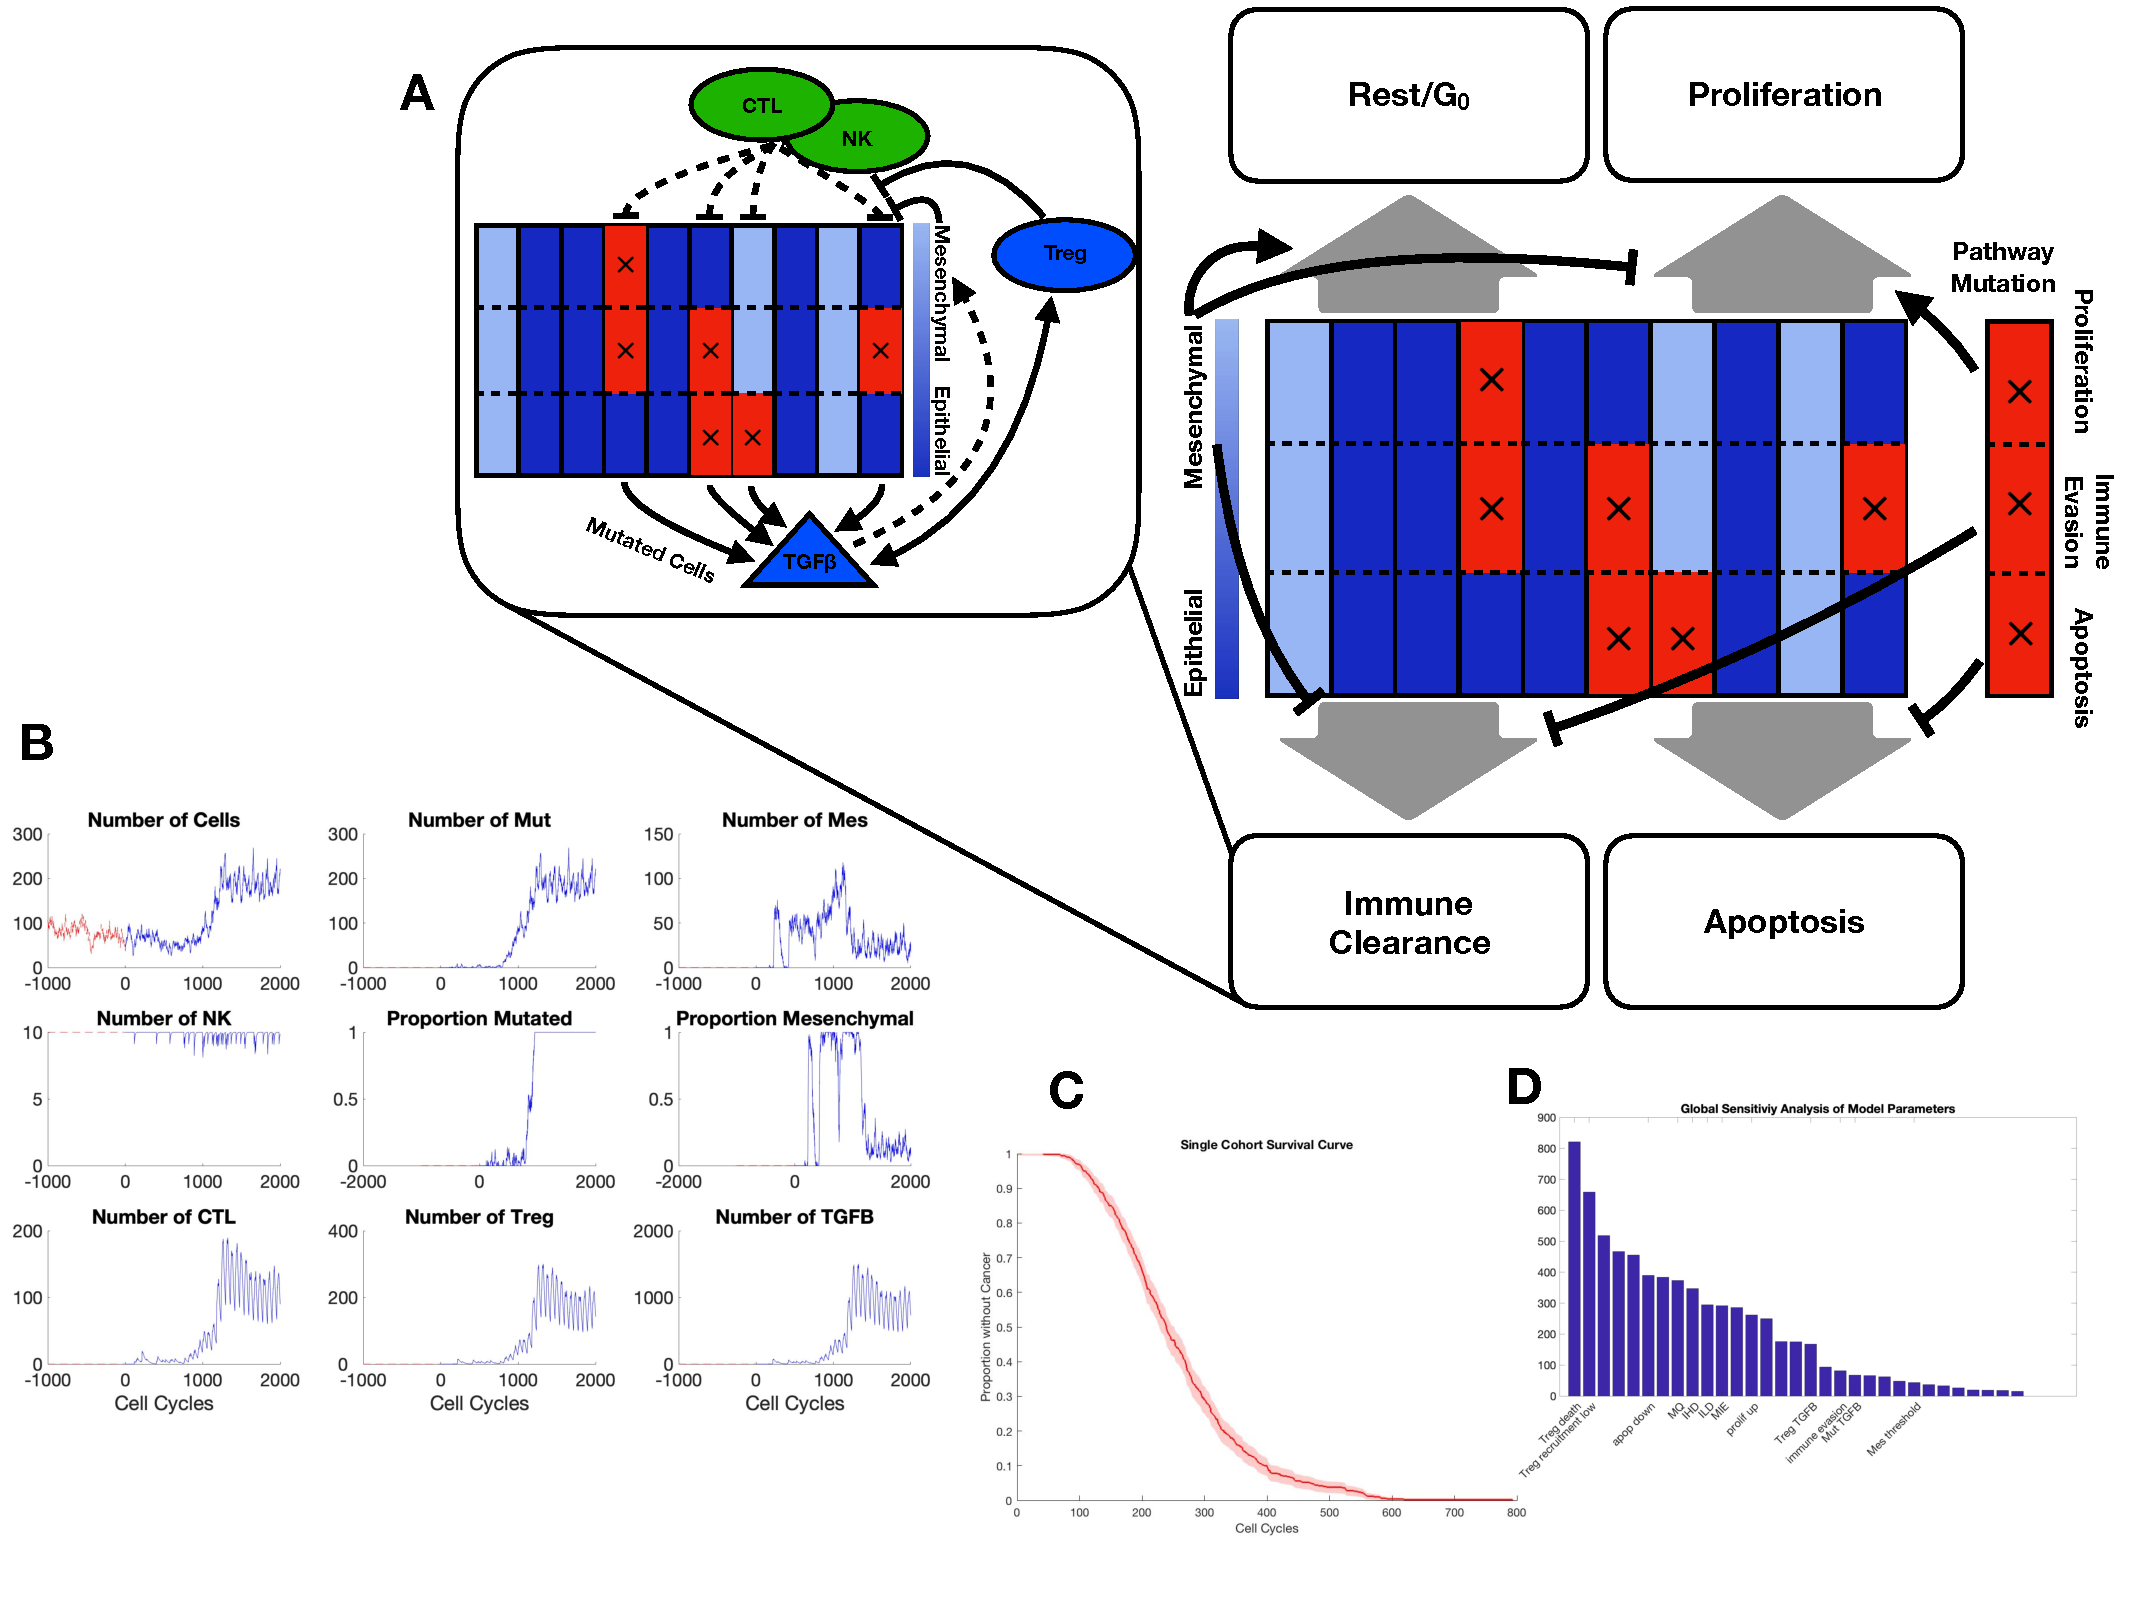
\includegraphics[width=\columnwidth]{Figure1/Figure1.pdf}}
\caption{A. Schematic depiction of the model with blue/red denoting non-mutated/mutated cells in the agent-based model. In each cycle, the fate of a cell is regulated by the EMT state of the cell and by any pathway mutations harbored. Inset shows major processes of immune system regulation on the tissue cells. The parameters used in this model can be found in the Supplementary material. Unless otherwise stated, parameter values are assumed to be those found in the Supplement. \tcr{Thoughts on the wording here? Once I have the table, I will use the name of that table.}
B. Example simulation of the dynamics of a one patient; warmup period is shown in red.
The inflammation cycling scheme is graphically represented above the patient dynamics.
C. Example survival curve for one cohort of patients with basal parameter values.
%A Should I list out all parameter values? A subset? Or refer to supplement for base parameter values?
D. Global sensitivity analysis of model parameters using the Morris one-step-at-a-time method.}
\label{fig:ModelIntro}
\end{figure}

\begin{figure}[H]
\center
\frame{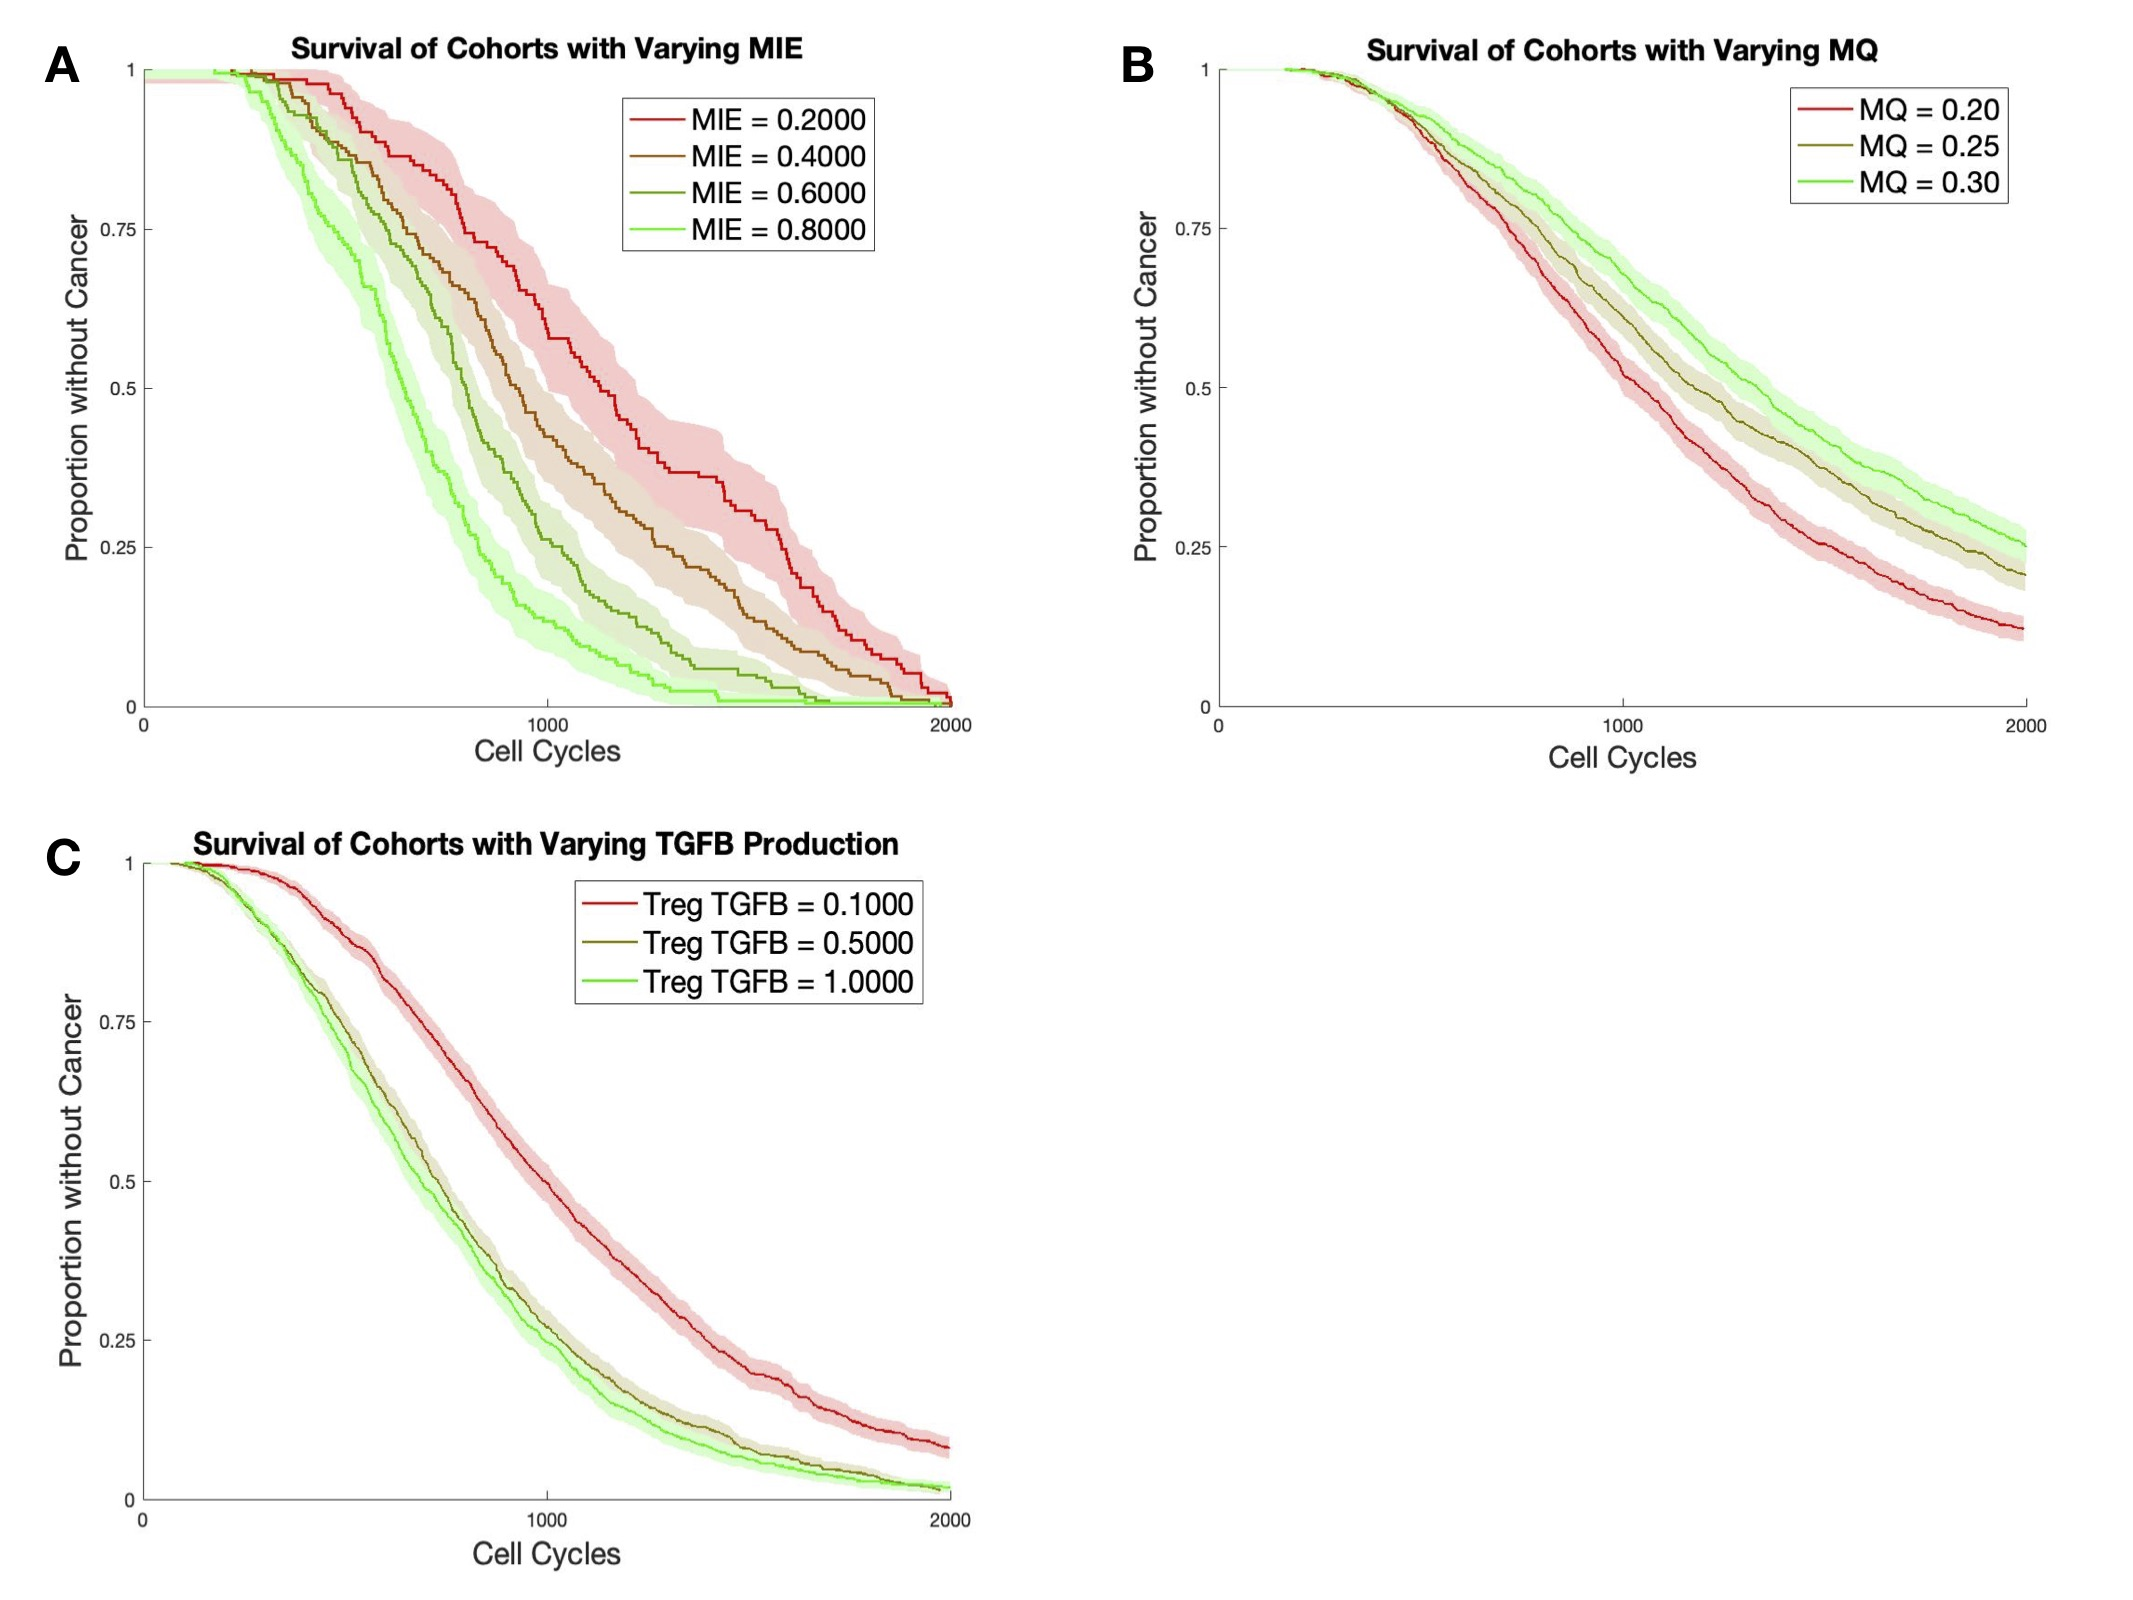
\includegraphics[width=\columnwidth]{Figure2/Figure2.jpg}}
\caption{Global sensitivity analysis of model parameters using the Morris one-step-at-a-time method.}
\label{fig:MOAT}
\end{figure}

\subsection{A multiscale agent-based model of EMT-immune-tissue cell interactions and tumorigenesis}\label{ExplModel}
We begin by studying the model under baseline conditions to assess how its various components interact and effect the overal probability of tumorigenesis (Time to Cancer). In Figure \ref{fig:ModelIntro}A a schematic description of the model is shown. Within a single cell cycle, different choices are available to a cell and these are influenced by pathway mutations or EMT. For example, if a cell undergoes EMT, the probability that is will proliferate is reduced. Also shown are the different means by which the immune system acts on the tissue cells (\ref{fig:ModelIntro}A Inset). The NKs and CTLs attempt to clear out mutated tissue cells and deactivate upon successfully carrying out this cytotoxic function. The Tregs inhibit this cytotoxic activity. In addition, Tregs release TGF-$\beta$ which helps recruit more Tregs and also drives EMT.
%A \tcr{TGF-$\beta$ is [describe briefly action of each immune cell type]}  --Adam: Is this good?

For a typical {\it in silico} patient (see Figure \ref{fig:ModelIntro}B), after the warmup period, some cells mutate but are cleared before establishing a tumor. However, eventually one mutated cell is able to establish a growing tumor before being cleared. This happens around cell cycle 1000. At this point, the adaptive immune system (CTLs and Tregs) are being heavily recruited and TGF-$\beta$ is peaking. The number of mesenchymal cells grows with the increased TGF-$\beta$, but decreases rapidly after the tissue cells are entirely mutants. Interestingly, this return to a more epithelial phenotype occurs even as TGF-$\beta$ reaches its maximum value for the simulation.
%\tcr{[What happens??]}
The inflammation cycling scheme for this patient is shown at the top of Figure \ref{fig:ModelIntro}B and is repeated throughout, including during the warmup.
We will return to this shortly.

%\tcr{[What is?]} 
At cell cycle number 841 the proportion of mutated cells reaches 50\% and so the model marks the patient as having a Time to Cancer of 841, or 630.75 days. 
At the same time as mutated cells are taking over, many cells transition to a mesenchymal phenotype.
After the Time to Cancer, the mutated cells continue their rapid growth and soon make up 100\% of the cells.
Meanwhile, all the cells become mesenchymal for a short duration before most transition back to an epithelial state.

Considering the immune populations, we see that the NK population is approximately constant, while the lymphocyte populations grow quickly and dwarf the NK population following the accumulation of mutations.
The lymphocyte populations exhibit oscillatory behavior, however note that this is not due to intrinsic dynamics but rather due to the inflammation scheme that this patient is undergoing: 
the patient alternates between 30 cell cycles of high inflammation and 60 cell cycles of low inflammation.
In each of these periods periods, the lymphocyte populations increase or decrease rapidly in accordance with the inflammation.

We next consider a cohort of $N=500$ patients, and simulate the survival curve for these patients (Figure \ref{fig:ModelIntro}C). We see that all patients survive for approximately 100 cell cycles (75 days), before a time period where the cancer onset rate is roughly constant, between the approximate range of ($T = 100, T = 300$).

\subsection{Identification of key model parameters via Morris global sensitivity analysis}\label{SensAnalysis}
To assess the sensitivity responses \tcr{Is this the right phrasing? It sounds funny to me, but I see Adam chose this wording.} produced by the model with respect to the 31 model parameters, a Morris one-step-at-a-time (OAT) algorithm was implemented.
The results of Morris OAT sensitivity analysis are shown in Figure \ref{fig:MOAT}. A subset of parameters demonstrate much higher levels of sensitivity than others.
The two most influential according to this analysis are the death rate and the recruitment rate of Treg cells, this is most likely due to the dual roles Treg cells play in both suppressing the cytotoxic effects of other immune cells and secreting TGF-$\beta$, which drives EMT.
This ties Treg cells to all three components of the model.
Since below we seek to separate the effects of different model components, we do not choose the parameters influencing Treg cells for further analysis below.

Any of the parameters in the table which include the word ``low'' are parameters that govern the model in a low inflammatory state.
With the exception of ``prolif up'', all parameters that end in ``up'' or have `U' at the end of their abbreviation, are the factors by which these parameters change when the system switches from low to high inflammation.
The IHD and ILD parameters determine the duration of high and low inflammation, respectively.
A cell with mutated pathways will be affected by the ``apop down'', ``prolif up'', and ``immune evasion'' parameters, depending on which pathways are mutated.
The mesenchymal cells are influenced by the MGA and MIE parameters.
Finally, $\sigma$, $k_\text{EMT}$, TGFB$_{max}$, and $\gamma_\text{EC50}$ all control how cells transition between the epithelial and mesenchymal states.

We want to better isolate the effects of EMT on these dynamics, so parameters such as MIE and MGA are of interest.
In addition, inflammation parameters dictating the cycling scheme are important to study\tcr{REF}: we find that there are also high sensitivities in this model to these parameters.
In terms of Treg cells, their secretion of TGF-$\beta$ is highly significant and we will also study it further.



\subsection{Mesenchymal phenotypic properties dramatically change survival outcomes}\label{MesPars}
The two quantities that change when a cell transitions to a mesenchymal state are its immune evasion and its proliferation rate, MIE and MGA, respectively.
Both parameters are proportions between 0 and 1 with higher values indicating more extreme expression of mesenchymal properties.
MIE is the proportional reduction of the probability a mutated mesenchymal cell will undergo immune clearance in a given cycle.
MGA, which stands for mesenchymal growth arrest, is the proportional reduction in any mesenchymal cell of its chance to proliferate in a given cell cycle. 
The reduction in proliferation probability corresponds with an equal increase in probability for resting during that cell cycle.  
%\tcr{[briefly redefine what these terms do]}
Also involved in the EMT process, is the cytokine TGF-$\beta$, which upregulates EMT.
By the Morris OAT analysis presented in Section \ref{SensAnalysis}, these three parameters do have large impacts on survival outcomes and each warrant exploration.


We found that as the level of mesenchymal immune evasion (MIE) increases, Time to Cancer decreases ( Figure \ref{fig:FirstSurvivalCurves}A).
This result holds for all parameter sets studied, and indicates the simple relationship that mesenchymal immune evasion has with Time to Cancer.
As this subpopulation of the tumor becomes more resistant to immune clearance, the tumor as a whole grows more resilient and thus will grow faster.
These results are summarized by Figure \ref{fig:FirstSurvivalCurves}A.

\begin{figure}[H]
\center
\frame{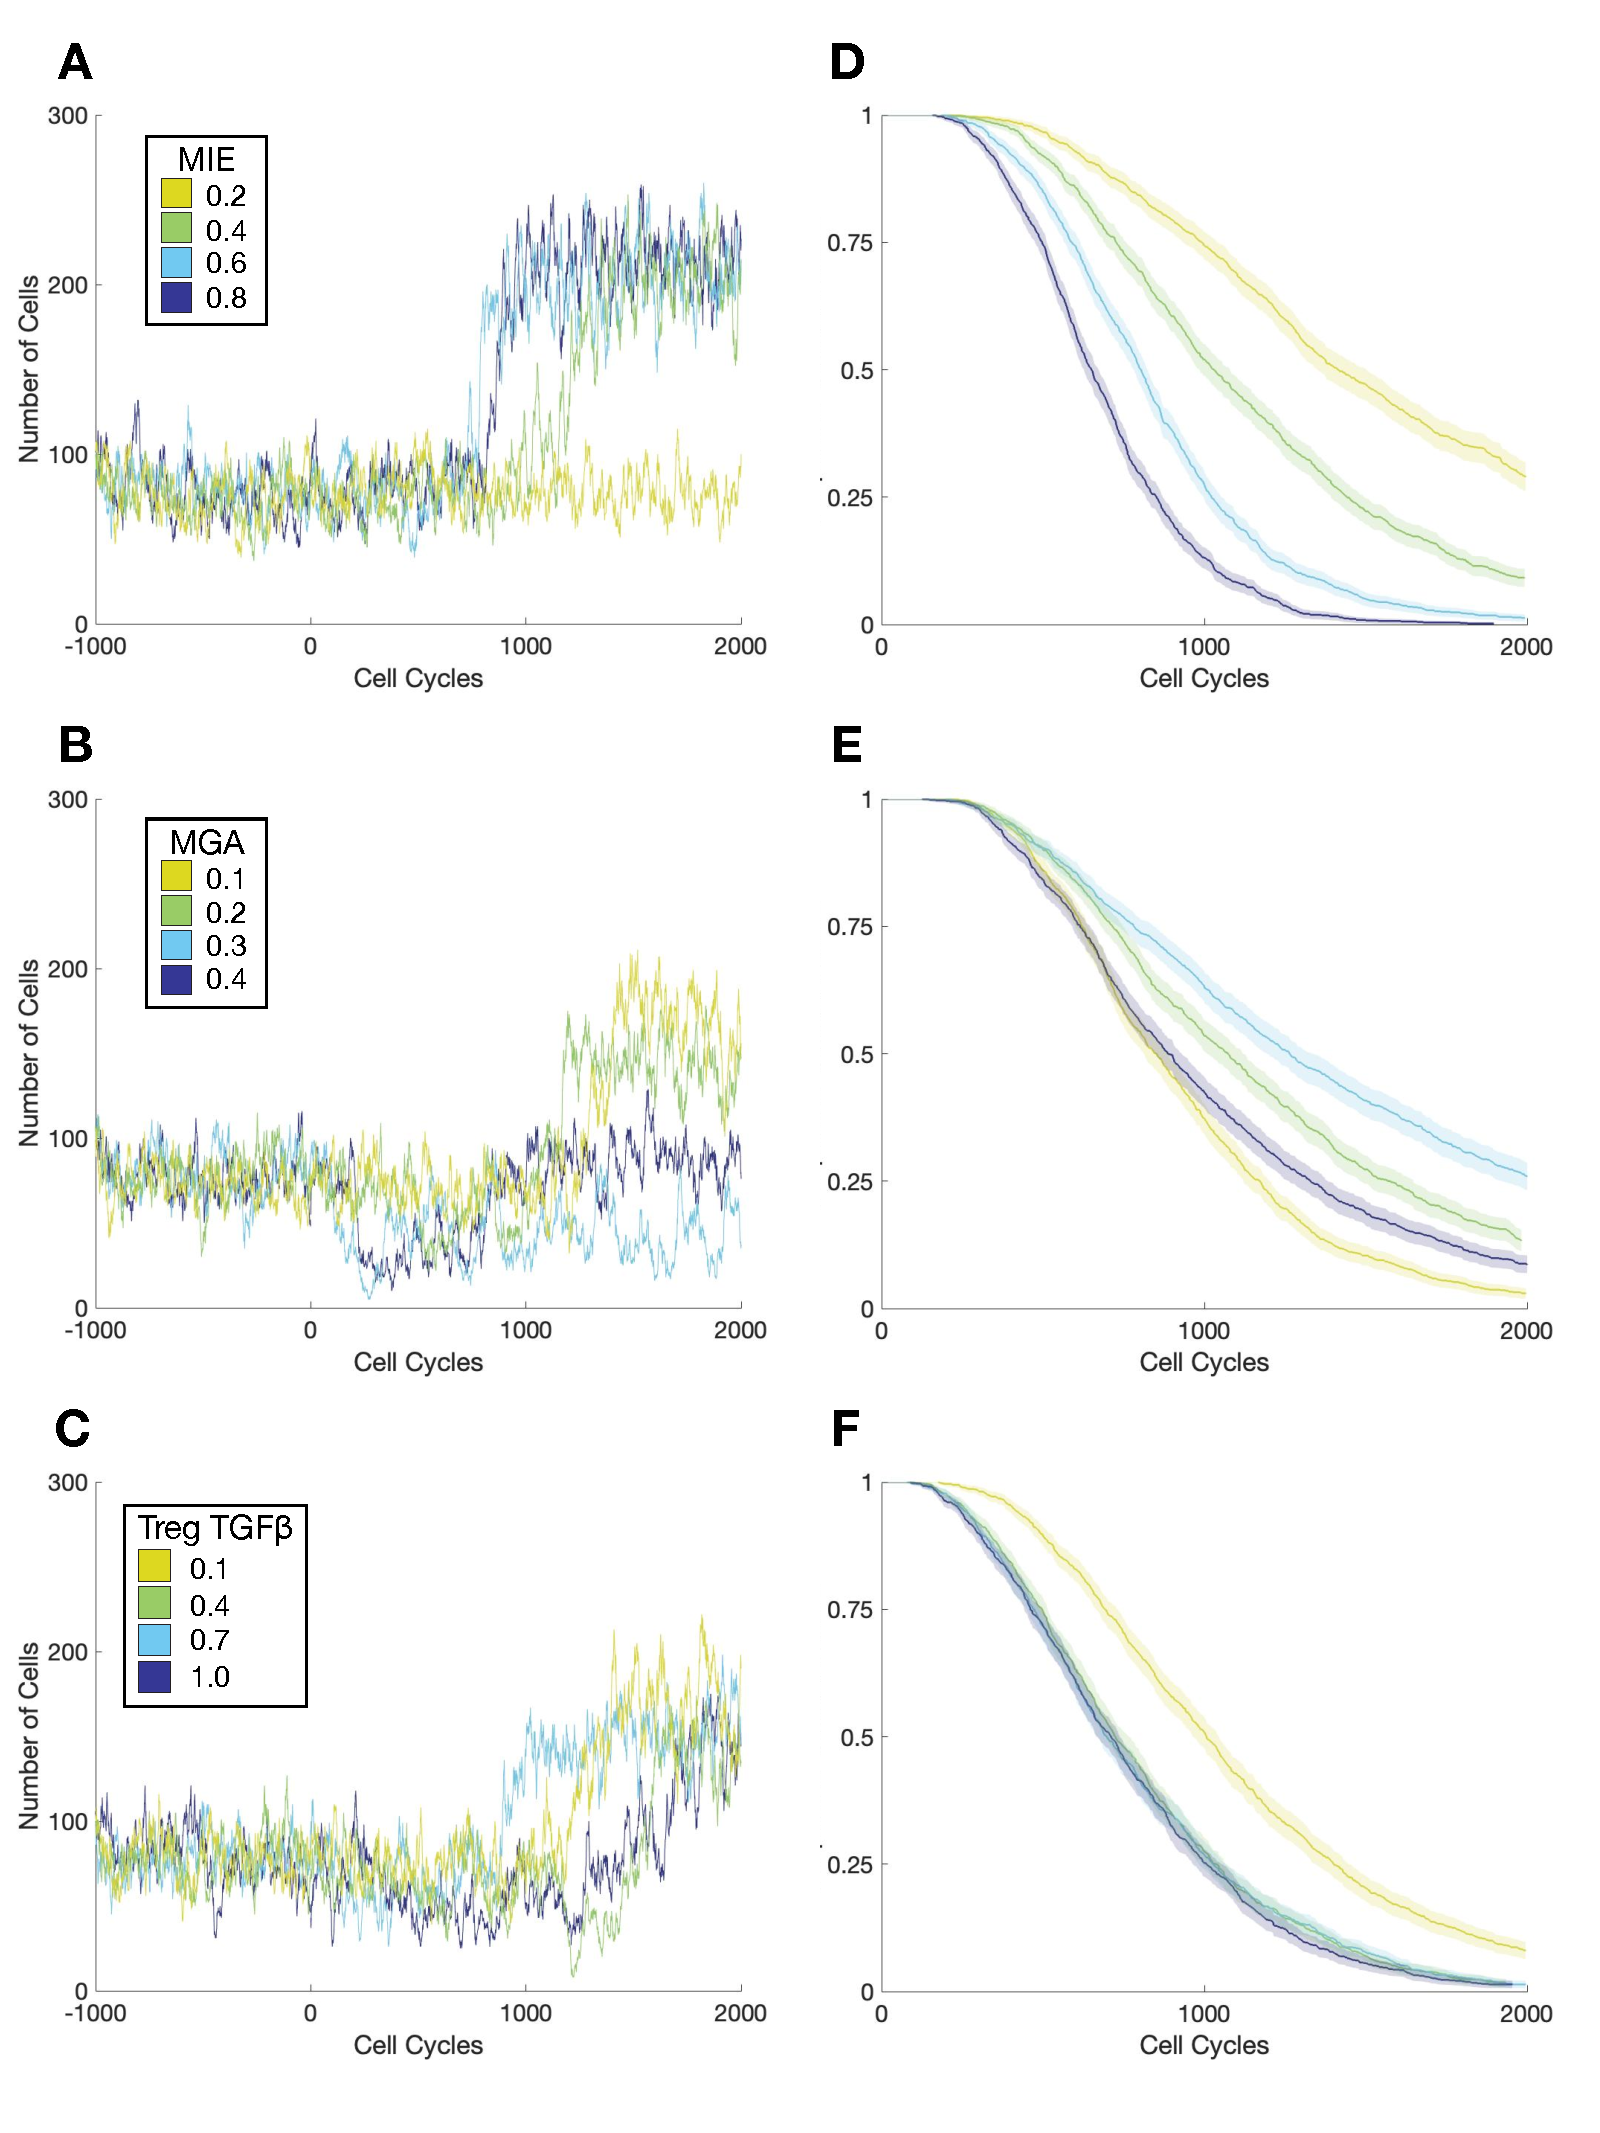
\includegraphics[width=\columnwidth]{Figure3/Figure3.pdf}}
\caption{
A-C. Trajectory of one patient per cohort followed from warmup through 2000 cell cycles.
\tcr{OK to do A-C like this?}
D. Increasing MIE decreases Time to Cancer. 
E. Increasing MGA increases Time to Cancer.
F. Increasing Treg TGF-$\beta$ production results in decreased Time to Cancer.
%% {\color{red} Cox regression or KM test statistics to be computed to demonstrate the significance of this claim.}
}
\label{fig:FirstSurvivalCurves}
\end{figure}

Second, as the rate of mesenchymal growth arrest (MGA) increases, Time to Cancer increases, i.e. lower proliferation rates for mesenchymal cells slow down cancer growth (Figure \ref{fig:FirstSurvivalCurves}B).
This is not immediately intuitive, since the decreased proliferation rate affects both mutated and non-mutated tissue cells.

Third, TGF-$\beta$ can be varied in two ways: the production by mesenchymal cells and the production by Treg cells.
In Figure \ref{fig:FirstSurvivalCurves}C, the results of varying Treg TGF-$\beta$ production are shown, indicating that an increased Treg TGF-$\beta$ production leads to a shorter Time to Cancer.
The two main ways in which TGF-$\beta$ influences the system is in recruitment of Treg cells and in pushing tissue cells to a mesenchymal phenotype.
Treg cells are modeled as tumor-protective and thus increasing their number will naturally decrease Time to Cancer.
Mesenchymal cells are more likely to evade the immune system, so pushing the system towards an overall more mesenchymal phenotype will better protect the cancer and decrease the Time to Cancer.


\subsection{A key EMT regime maximizes cancer-free survival time under chronic inflammation}\label{KeyEMT}
Given the relevance of the inflammatory state of the tumor microenvironment (TME), we explore the effect of varying the inflammation state of the patient on survival.
In simulations, we assign some cohorts permanently low inflammation levels, some permanently high levels, and some variable inflammatory schemes.
For those cohorts with a permanently high inflammatory state, the relationship between the mesenchymal parameters and the Time to Cancer is monotonic.
However, when there are periods of a low inflammatory state, then intriguingly the connection between MGA and Time to Cancer becomes concave down with a local maximum around 0.3.
This can be seen in the top two groups of Figure \ref{fig:VaryINFL_and_MesPars}D: the MGA=0.3 cohorts both took longer to cancer than their neighbors.
What this indicates is that if the growth arrest of mesenchymal cells can be controlled, then they could be manipulated in such a way as to increase the Time to Cancer.
Even if the patient is presenting a chronically high inflammatory state, anti-inflammatories could be administered which would create the periods of low inflammation our model predicts as necessary for seeing these changes.
Reducing the inflammatory state of the TME three weeks out of every nine would be sufficient to make the control of mesenchymal proliferation an effective anti-cancer strategy.
%Furthermore, even if the patient is presenting a permanent high inflammatory state, medications could be prescribed which would lower the inflammatory state temporarily and thus create a similar cycling inflammatory regime which could be taken advantage of in the same way. \tcr{what does this mean? how?}

\begin{figure}[H]
\center
\frame{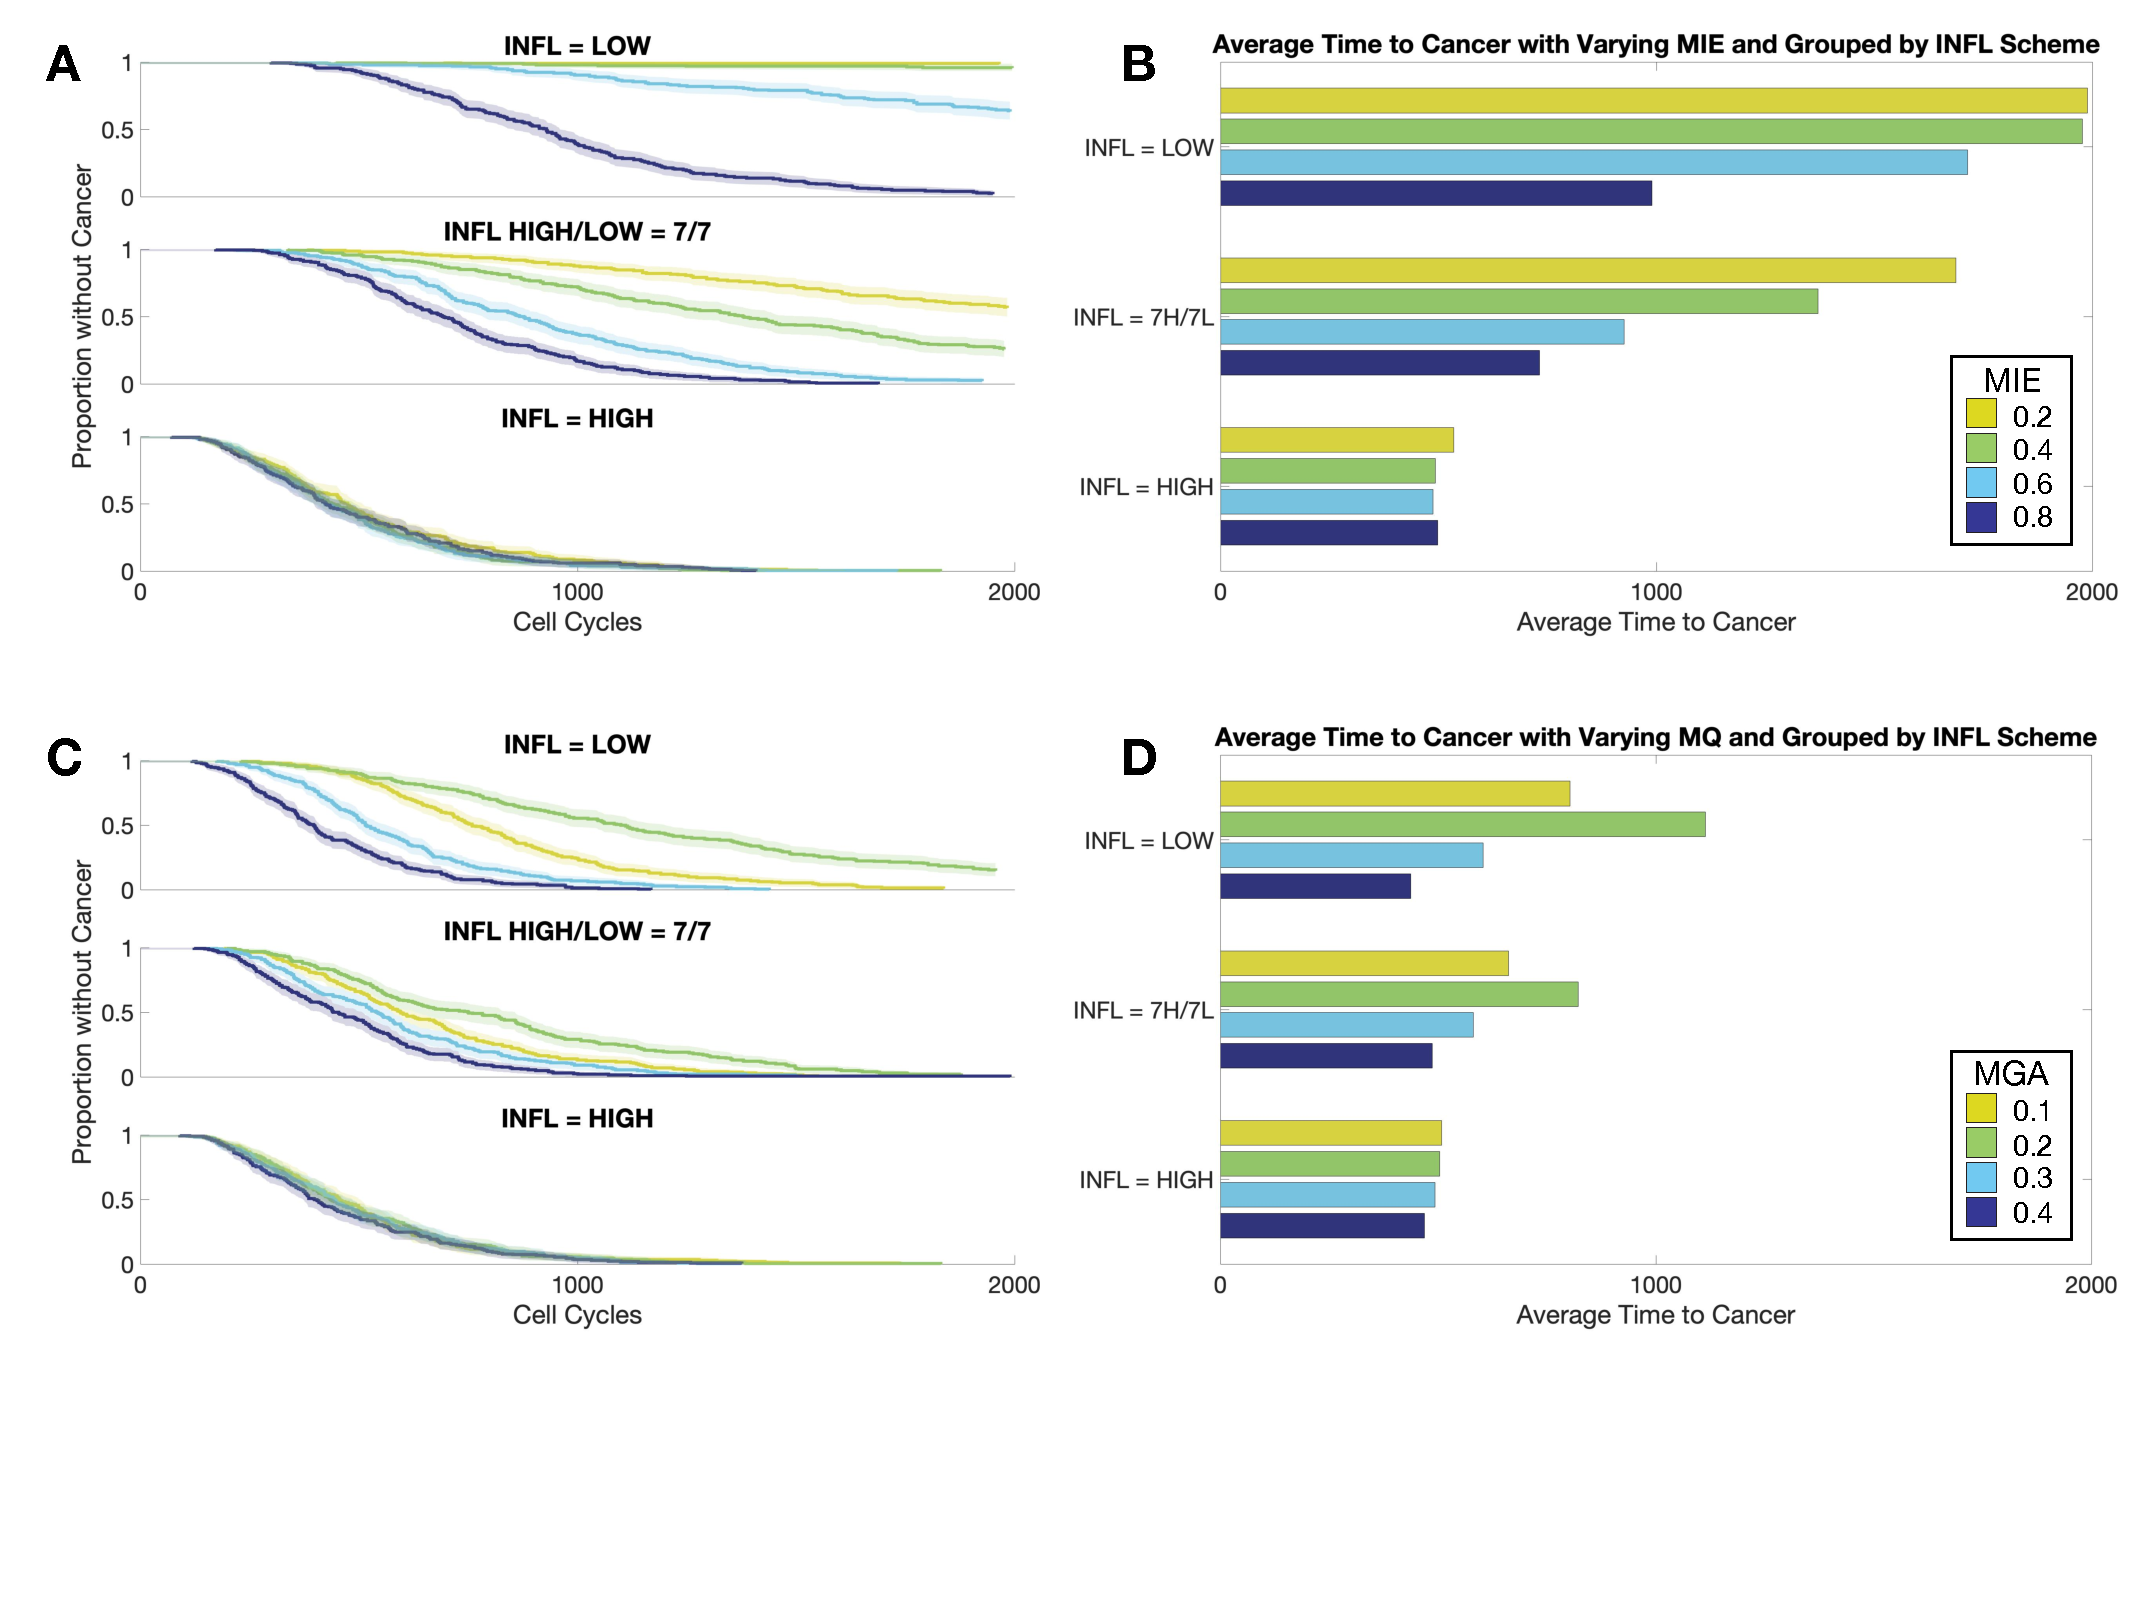
\includegraphics[width=\columnwidth]{Figure4/Figure4.pdf}}
\caption{A. Survival curves for various inflammation cycling schemes. In the top two plots, the Time to Cancer decreases as MIE increases. In the bottom plot, there is no significant difference in survival.
B. The average Time to Cancer for each cohort.
C. Survival curves for various inflammation cycling schemes. In the top two plots, the Time to Cancer reaches a maximum value somewhere near MGA = 0.3. In the bottom plot, there is no significant difference in survival.
D. The average Time to Cancer for each cohort.}
\label{fig:VaryINFL_and_MesPars}
\end{figure}

Contrast this with what happens when MIE is varied for different inflammation cycling schemes.
Regardless of the cycling scheme, the relationship between Time to Cancer and MIE is monotonic.
In the case that the inflammatory state is permanently high, MIE has no significant effect on Time to Cancer.
On the other hand, when the patient experiences at least some time in a low inflammatory state, an increase in MIE results in a decrease in Time to Cancer.
This indicates that mitigating a chronic inflammatory state is a necessity for increasing survival, and once that has been achieved, even to a small degree, then therapies which reduce mesenchymal immune evasion will gain efficacy.


% \subsection{Heat Map of MIE vs MGA}
\subsection{Analysis of TCGA data in comparison with model predictions suggests that mesenchymal phenotypes reduce cancer-free survival probability}\label{tcga}

To further analyze the effects on tumorigenesis of the mesenchymal properties of immune evasion (MIE) and growth arrest (MGA), we study the joint density plot detailing the effects of each of these parameters on the Time to Cancer (Fig. \ref{fig:MIEvsMGA}). We found that over the full range of values of MGA considered, increasing the MIE decreases the Time to Cancer. However, for any given value of mesenchymal immune evasion, there is a value of mesenchymal growth arrest that maximizes the Time to Cancer. Moreover, this optimal value increases with MIE. 

\begin{figure}[H]
\center
\frame{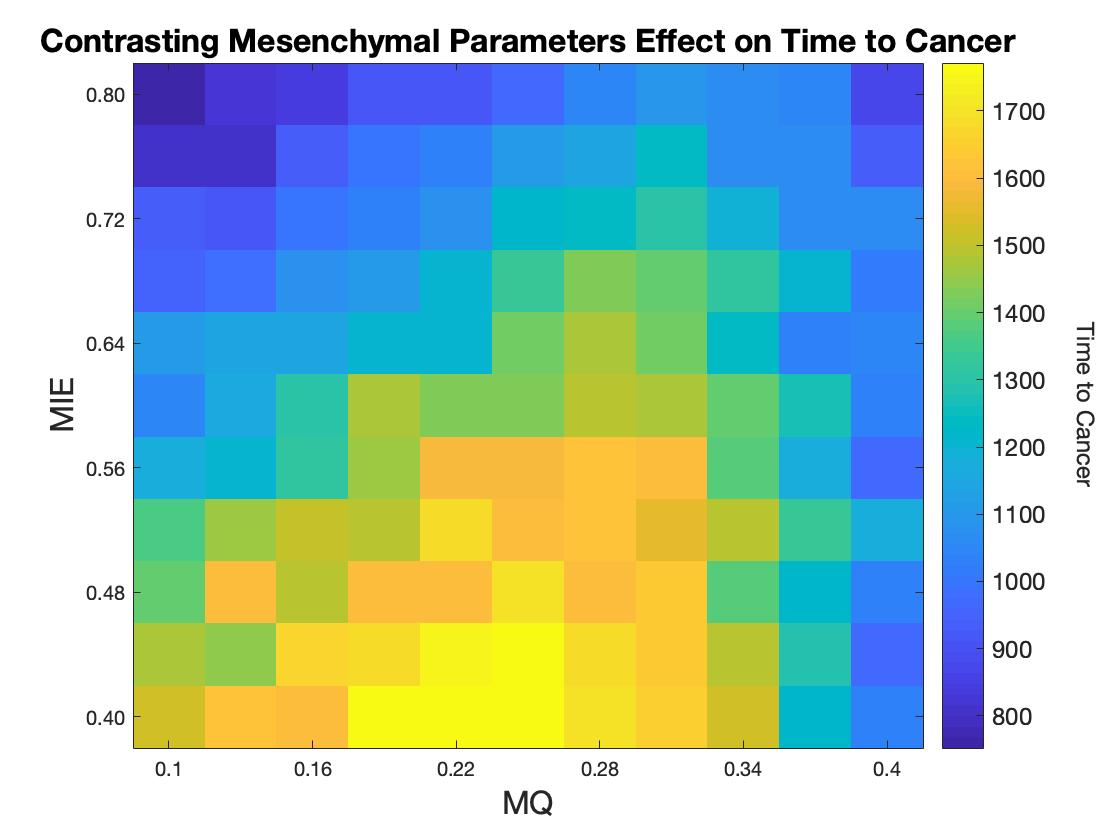
\includegraphics[width=\columnwidth]{Figure5/MIEvsMQ.jpg}}
\caption{Heat Map contrasting the effects of MIE and MGA on Time to Cancer. Increasing MIE always decreases Time to Cancer, but MGA is non-monotonically linked to Time to Cancer.}
\label{fig:MIEvsMGA}
\end{figure}

To compare these model predictions with experimental studies, we performed analysis of data from The Cancer Genome Atlas (TCGA) database to study the effects of immune and EMT interactions on prognosis of cancers for which inflammation is known to play an important role, such as colonic or pancreatic cancers (REFS). We selected pancreatic cancer to investigate, and used gene ontologies as a measure of the of effects of inflammatory or EMT processes on survival. In Fig. \ref{fig:tcga} we plot survival curves for two cases: either clustering only on EMT, or on both EMT and inflammation signatures. We see that in both cases, survival is significantly affected by the gene ontology signature, but importantly, the presence of both EMT and inflammation signatures has a greater impact on survival than the effects of EMT alone.  



\begin{figure}[H]
\center
\frame{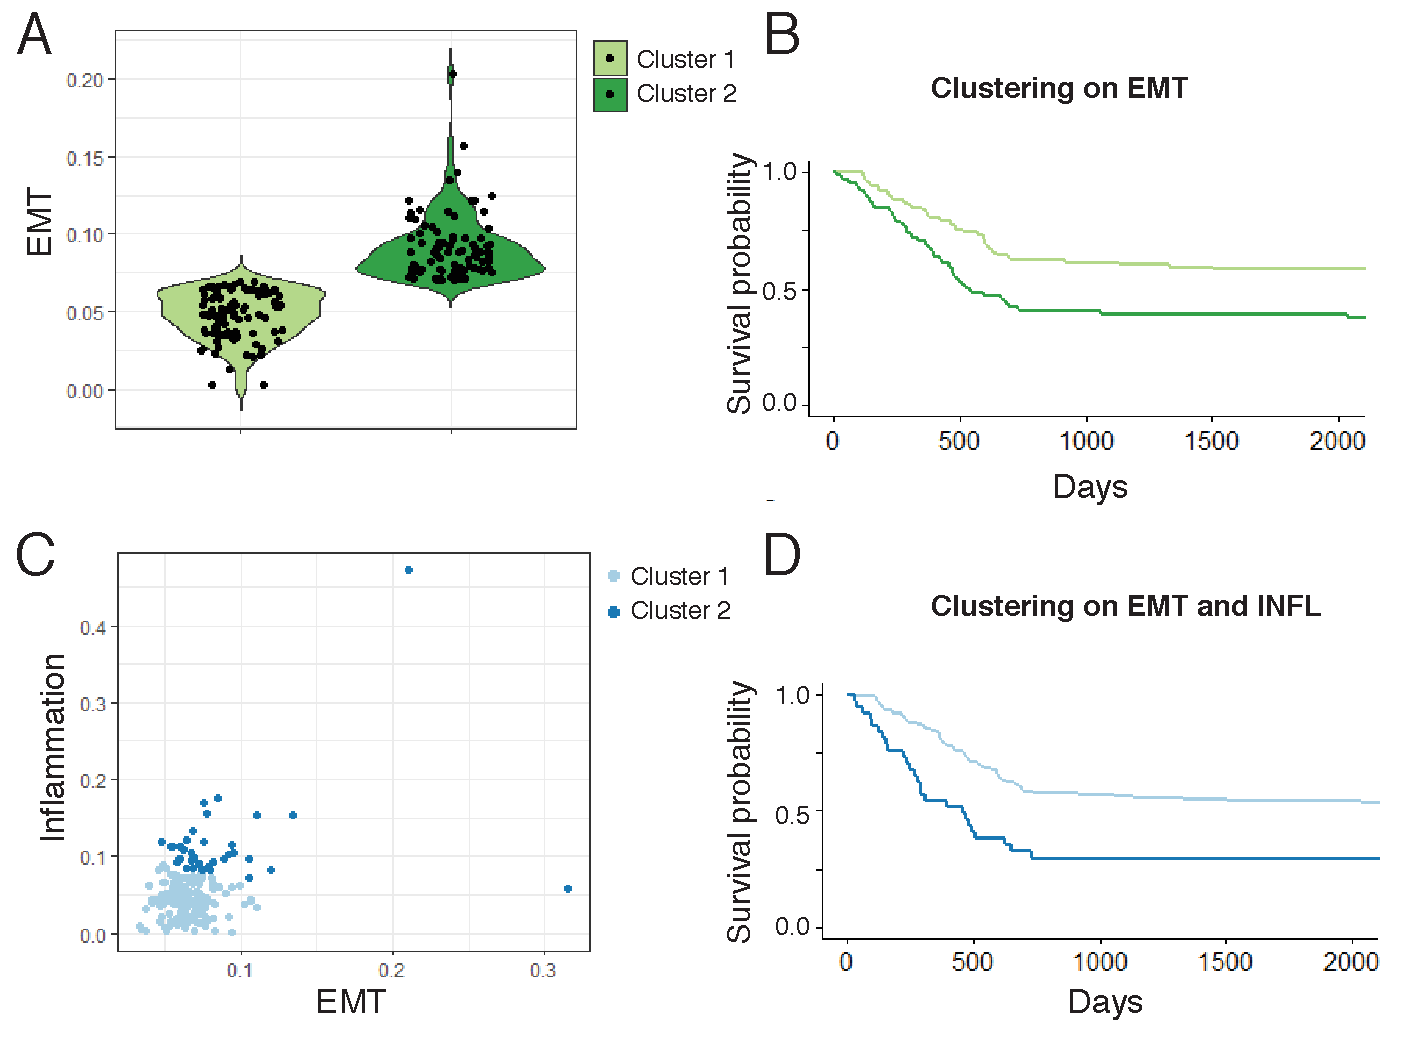
\includegraphics[width=\columnwidth]{FigTCGA.pdf}}
\caption{A. K-means clustering of pancreatic cancers using gene ontology terms indicative of an EMT signature ($k=2$). B. Survival plots corresponding to the clustering on EMT. C. K-means clustering of pancreatic cancers using gene ontology terms indicative of EMT and Inflammation signatures ($k=2$). D. Survival plots corresponding to the clustering on EMT and inflammation.}
\label{fig:tcga}
\end{figure}



%%%%%%%%%%%%%%%%%%%%%%%
%                      DISCUSSION                       %
%%%%%%%%%%%%%%%%%%%%%%%

\section{Discussion}\label{Discussion}
In building this model, we set out to better understand how the immune system and the EMT spectrum would affect Time to Cancer results from previous work.
What we found is that altering many of the processes have predictable results: increasing mesenchymal immune evasion, decreasing mesenchymal growth arrest, and increasing Treg TGF-$\beta$ production all lead to shorter Times to Cancer.
However, when the inflammation of the TME is accounted for, some of these changes to the system have less predictable outcomes.
The most intriguing is that periods of low inflammation lead to mesenchymal growth arrest having an optimal value for maximizing Time to Cancer.



%In addition, I could discuss the implications from the TGF-$\beta$ section.
%Any discussion on this topic, however, would need to acknowledge that regulation of TGF-$\beta$ might also have other, serious side effects, especially if the treatment is not local.
%However, that might also be true for the inflammatory results.
%In light of this, it might be good to include a new section on how TGF-$\beta$ production's influence on Time to Cancer is influenced by the inflammatory cycling scheme.



%%%%%%%%%%%%%%%%%%%%%%%
%                     CONCLUSION                      %
%%%%%%%%%%%%%%%%%%%%%%%

\section{Conclusion}\label{Conclusion}
The interactions of the immune system and cancer remain a promising avenue of research.
Including more diverse aspects of the TME and the tumor itself make the challenge that much harder but also that much more promising.
As we begin to understand how processes such as EMT factor in to these complex interactions, we can begin to respond clinically to better improve patient outcomes.
Here, we saw {\it in silico} evidence of an optimal value for a property of mesenchymal cells that would maximize Time to Cancer.
There is still much work to be done further isolating this effect in computer simulations and further verifying this effect and exploring further ways EMT can influence tumor progression.
This model explored much more than mesenchymal growth arrest, so a simpler model could make this point clearer.
On the other hand, models which incorporate more distinctions between epithelial and mesenchymal cells could give better clarity on the relative importance of these and reveal a fuller picture about how a mesenchymal subpopulation affects cancer outcomes.

%A Adam, do you know of any?
The authors are not aware of current treatments that specifically target mesenchymal growth arrest, influencing it in one direction or another.
%
Based on these results, this could prove to be a promising direction for research, in particular for cancers in which it is known that mesenchymal cells are present and active within the tumor.
The greatest challenge in translating the information here to the clinic, apart from creating the drugs, would be discovering the ideal growth rate for mesenchymal cells within each patient and how other patient-specific data will influence this result.

Progress in cancer treatment has always proven attainable even despite great challenges, for which the complexity of the disease is often responsible. As we move forwards, it is these very complexities that we will be able to better exploit to eradicate or control the disease.


\bibliography{mybib}{}
\bibliographystyle{siam}

\end{document}